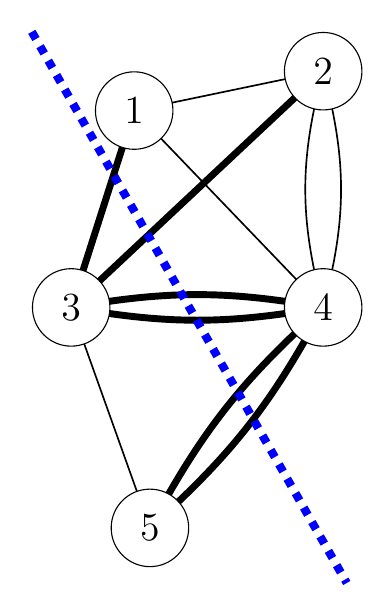
\begin{tikzpicture}[
    % Define Styles
    vertex/.style={
        circle,
        draw,
        minimum size=28pt,
        inner sep=0pt,
        fill=white,
        font=\Large\rmfamily
    },
    thickedge/.style={
        draw,
        line width=2.5pt
    },
    thinedge/.style={
        draw,
        semithick
    },
    cutline/.style={
        draw,
        blue,
        dashed,
        line width=3pt
    }
    ]

    % Define Coordinates
    \coordinate (c3) at (0, 0);       % Node 3 (Left Middle)
    \coordinate (c1) at (0.8, 2.5);   % Node 1 (Top Left)
    \coordinate (c2) at (3.2, 3.0);   % Node 2 (Top Right)
    \coordinate (c4) at (3.2, 0);     % Node 4 (Right Middle)
    \coordinate (c5) at (1.0, -2.8);  % Node 5 (Bottom)

    % Draw Edges

    % Edges connected to Node 1
    \draw[thinedge] (c1) -- (c2);
    \draw[thickedge] (c1) -- (c3);
    \draw[thinedge] (c1) -- (c4);

    % Edges connected to Node 2
    \draw[thickedge] (c2) -- (c3);
    % Double curved thin edges between 2 and 4
    \draw[thinedge] (c2) to[bend right=15] (c4);
    \draw[thinedge] (c2) to[bend left=15] (c4);

    % Edges connected to Node 3
    \draw[thickedge] (c3) to[bend right=10] (c4);
    \draw[thickedge] (c3) to[bend left=10] (c4);
    \draw[thinedge] (c3) -- (c5);

    % Edges connected to Node 4
    \draw[thickedge] (c4) to[bend right=10] (c5);
    \draw[thickedge] (c4) to[bend left=10] (c5);

    % Nodes
    \node[vertex] (n1) at (c1) {1};
    \node[vertex] (n2) at (c2) {2};
    \node[vertex] (n3) at (c3) {3};
    \node[vertex] (n4) at (c4) {4};
    \node[vertex] (n5) at (c5) {5};

    % Blue Cut Line
    \draw[cutline] (-0.5, 3.5) -- (3.5, -3.5);

\end{tikzpicture}